\chapter{Excitación de átomos por impacto de electrón}

%=======================================================================
\section{Introducción}
\label{sec:intro}

El espectro de átomos complejos en diversos estados de ionización son 
emitidos por objetos astronómicos, la corona solar, nebulosas, quasars, 
etc, y también en descargas en laboratorios terrestres. La interpretación
de dichas observaciones requiere de una extensa variedad de datos 
atómicos. Los cálculos de niveles de energía son utilizados como una guía
para identificar las líneas espectrales observadas, mientras que sus 
intensidades requieren la determinación de secciones eficaces 
colisionales y fuerzas de oscilador. 
El modelado de diagnóstico espectroscópico de plasmas astrofísicos y de 
laboratorio tiene un gran apetito por los coeficientes de tasa de 
excitación de impacto de electrones, ya que determinan en gran medida la 
distribución de la población emisora dentro de un estado de carga. El 
método de acoplamiento cercano puede, en principio, proporcionar datos 
de excitación entre todos los estados objetivo incluidos en su expansión.

La descripción precisa de la excitación por impacto de electrones de los 
iones atómicos sigue siendo una de las tareas más desafiantes para los 
métodos no perturbativos más avanzados, tales como el acoplamiento 
cercano convergente (\acs{ccc})~\cite{Bray:92}, el acoplamiento cercano 
de matriz R (\acs{rm})~\cite{Burke:75} y el acoplamiento cercano 
dependiente del tiempo (\acs{tdcc})~\cite{Pindzola:07}; aún en la 
actualidad, cuando se cuentan con máquinas con enorme poder computacional. 
Por otro lado, la importancia de la correcta representación de la 
estructura atómica al describir la excitación por impacto de electrones 
ha sido estudiada y demostrada usando diversos métodos de acoplamiento 
cercano (\acs{cc})~\cite{Bartschat:04,Zatsarinny:16,Be_Ballance:03} para 
un gran número de blancos. Particularmente, en blancos neutros y de bajo 
grado de ionización existe un gran número de trabajos de 
investigación~\cite{Ballance:03,Badnell:03,Mitnik:03} que han demostrado 
la importancia del acoplamiento al continuo del blanco para describir 
correctamente este proceso. Sin embargo, la determinación de una adecuada 
representación del blanco no es condición suficiente. La apropiada 
resolución del problema colisional requiere además un amplio conocimiento 
sobre el método y, en general, grandes recursos computacionales.

En general, la precisión de los cálculos de estructura del blanco aumenta 
con el número de configuraciones incluidas en la configuración de 
interacciones (\acs{ci}). Por otro lado, el Hamiltoniano del sistema de 
$N$ electrones es usualmente descrito en el marco de la aproximación de 
un electrón activo, lo que permite describir el blanco con potenciales 
radiales paramétricos. Así, la inclusión de nuevas configuraciones en el 
CI tiende a aumentar el número de parámetros que definen estos 
potenciales modelos e incrementa la complejidad de la optimización de la 
estructura. 

La estructura de blancos atómicos en procesos de impacto de electrón
son generalmente ajustados a mano, por un operador o tomador de 
decisiones (\acs{dm}) experimentado que tiene un gran conocimiento de la
naturaleza del ión y del proceso colisional a resolver. Este proceso de 
optimización es complejo y muy dificil de sistematizar. Sin embargo, un 
intento de sistematización del ajuste óptimo de los parámetros que 
definen la estructura atómica es proporcionado por el código 
\textsc{autostructure} (\acs{as}) de Badnell~\cite{Badnell:11}. El método 
numérico implementado en este caso es el método de Powell y ajusta los 
parámetros de escala que definen los potenciales modelo del blanco. Si 
bien este método proporciona una buena aproximación en la búsqueda de un 
mínimo global, éste requiere una correcta elección de semillas iniciales. 
En general, estos valores iniciales se buscan a partir de un mapeo de 
grilla, lo cual resulta computacionalmente costoso cuando se cuenta con 
un gran número de dimensiones. En el caso de AS, los valores iniciales de 
optimización son todos iguales a uno.

El trabajo desarrollado en este capítulo busca encarar el problema de 
optimización de estructura de blancos atómicos de forma sistemática, con 
mínima intervención de parte del DM. Para ello, recurrimos a herramientas
ampliamente usadas en el campo del aprendizaje automatizado (\acs{ml}). 
Particulamente, implementamos la optimización bayesiana (\acs{bo}) a 
través de procesos gaussianos (\acs{gp}). 

%=======================================================================
\section{Descripción del blanco}

En general, la función de onda de los blancos atómicos se expresa 
implementando el método de interacción de configuraciones (\acs{ci}); 
esto es,
\begin{equation*}
\Psi_i(\mathbf{r}) =
\sum_j^{N} c_{ji} \, \Phi_j(\mathbf{r})\,,
\end{equation*}
donde $N$ es el número de configuraciones electrónicas relevantes dentro
de la aproximación de interacción de configuraciones, y $\Phi_j$ son las
funciones de onda correspondientes a cada configuración. Dentro de la 
aproximación de electrón activo, la parte radial de las funciones de 
onda electrónicas se obtienen a partir de la resolución de la ecuación 
de Schr\"odinger radial de un electrón,
\begin{equation*}
\left[ \frac{1}{2} \frac{d^2}{dr^2} - \frac{l(l+1)}{2r^2} 
 + V_j^{\mbox{\scriptsize eff}}(\lambda_j,r)
 + E_j \right] P_j(r)=0\,,
\end{equation*}
donde $V_j^{\mbox{\scriptsize eff}}$ es un potencial modelo, que puede 
ser ajustado a partir de un parámetro de escala 
$\boldsymbol\lambda=\{\lambda_j\}$. 

\subsection{Potenciales modelo}

Existen diversos potenciales modelos que permiten el cálculo de la
estructura del blanco. En esta sección, nos centraremos en dos de los más 
usados: el potencial de Thomas-Fermi-Dirac-Amaldi (\acs{tfda}) y el 
potencial de orbitales tipo Slater (\acs{sto}) de Burgess. 

\subsubsection*{Potencial TFDA}

El potencial de Thomas-Fermi~\cite{Gombas:56,Eissner:69,Bautista:08} para 
una carga electrónica a una distancia $r$ del núcleo está dada por
\begin{equation}
V(r)=-\frac{2Z}{r}+\int_0^{r_0}\frac{2}{r_>} \rho(r')4\pi r'^2\,dr'\,,
\label{eq:Thomas-Fermi}
\end{equation}
donde $\rho(r)$ es la densidad de carga, $r_>$ es el mayor valor de entre
$r$ y $r'$, y $r_0$ es el radio de la superficie del átomo. El último
término del lado derecho surge de la aproximación clásica para una 
densidad de carga esféricamente simétrica. 

La energía total de este átomo está dada por la suma de sus valores 
cinéticos y potenciales; esto es,
\begin{equation}
E=\int_0^{r_0}\left[\frac{3}{5}(3\pi^2)^{2/3}\rho^{2/3}(r)-\frac{2Z}{r}
+\frac{1}{2}\int_0^{r_0}\frac{2}{r_>}\rho(r')4\pi r'^2\,dr'\right] 
\rho(r)4\pi r^2\,dr\,.
\label{eq:tot-ener-TF}
\end{equation}
Para valores de radio tal que $r\leq r_0$, la expresión de $E$ es 
minimizada para un valor de $\rho$ que satisface la relación
\begin{equation}
\left[3\pi^2\rho(r)\right]^{2/3}+V(r)-V_0=0\,, 
\end{equation}
donde, para un átomo aislado, la densidad electrónica debe ser cero en
$r=r_0$, y 
\begin{equation}
V_0=V(r_0)=-\frac{2(Z-N)}{r_0}
\end{equation}

Sin embargo, el modelo de Thomas-Fermi sólo contempla interacciones 
electrostáticas núcleo-electrón y electrón-electrón. Los efectos de 
intercambio electrónico fueron introducidos por Dirac. Sin embargo, la 
acción sobre cada electrón en este modelo está determinada por el campo 
resultante de los $N$ electrones; esto conduce al famoso problema de la 
auto-interacción de los electrones. Amaldi y Fermi corrigieron este 
inconveniente, y, ahora la ecuación (\ref{eq:tot-ener-TF}) es minimizada
para una de densidad de carga que está dada por
\begin{equation}
\rho(r)=\frac{1}{2\pi^2}\left\{\frac{1}{\pi}+\left[\frac{1}{\pi^2}+V_0-
V(r)\right]^{1/2}\right\}^3\,,
\end{equation}
y
\begin{equation}
V_0=-\frac{15}{16\pi^2}-\frac{2(Z-N)}{r_0}\,.
\end{equation}
Finalmente, se introduce un factor de escala en el potencial, tal que
\begin{equation*}
 V^{\textrm{TFDA}}(\lambda_i,r) = V(r/\lambda_i)\,.
\label{eq:TFDA-pot}
\end{equation*}

\subsubsection*{Potencial STO}

En el esquema del potencial de Burgess~\cite{Burgess:89}, se asume que 
cada uno de los electrones ligados se mueve en un potencial apantallado 
independiente, que es generado por una carga nuclear $Z$ y la 
distribución de carga de los $N-1$ electrones restantes. Se implementan 
orbitales de tipo Slater (\acs{sto}) $p_j(r)$ para calcular la 
contribución a esta distribución de carga por parte de los $q_j$ 
electrones en la $j$-ésima subcapa $n_jl_j$. Estos orbitales están dados 
por
\begin{equation}
p_j(r) = c\rho_j^n e^{-\rho_j/2}\,,
\end{equation}
donde $c$ es una constante de normalización, y 
\begin{equation}
\rho_j= \frac{2z_j\lambda_jr}{n_j}\,
\end{equation}
donde $\lambda_j$ es un parámetro de escala y 
\begin{equation}
z_j=Z-\frac{1}{2}\left(q_j-1\right)-\sum_{i<j} q_s\,.
\end{equation}
A una distancia $r$ del núcleo, cada uno de estos electrones genera un 
apantallamiento 
\begin{equation}
\frac{\left[\int_0^r p_j(\xi)\,d\xi +r\int_r^{\infty}
\frac{p_j(\xi)}{\xi}\,d\xi\right]}{\int_0^{\infty}p_j^2(\xi)\,d\xi}\,.
\end{equation}
Así, el potencial al que está sujeto un electrón fuera el la subcapa 
$i$-ésima es
\begin{equation}
V_i^{\textrm{STO}}(r)=-\frac{1}{r}\left\{Z-\sum_j(q_j-\delta_{ij})\left[1-
\frac{e^{-\rho_j}}{2n_j}\sum_{m=0}^{2n_j-1}\frac{(2n_j-m)}{m!}\rho_j^m
\right]\right\}\,.
\label{eq:STO-pot}
\end{equation}

\subsection{Potenciales de polarización}

En sistemas con ``núcleos electrónicos'' o \textit{cores} polarizables y 
pocos electrones de valencia, los efectos de correlación suelen ser 
significativos y deben ser considerados. En general, estos efectos son 
pronunciados en átomos alcalinos y alcalinotérreos, incrementando sus 
energías de ionización, contrayendo su capa de valencia, reduciendo 
polarizabilidades y fuerzas de oscilador~\cite{Muller:83}. 
Así, para obtener una representación precisa de las funciones de onda de 
átomos alcalinos y alcalinotérreos, es importante considerar no sólo las 
correlaciones de valencia, sino también las core-valencia 
\cite{Bartschat:04}. Una posible forma de incluir los efectos de 
correlación core-valencia está dado por la inclusión de potenciales de 
polarización de core semi-empíricos~\cite{Loughlin:88}.

\begin{comment} (sigue de Bartschat)
Although such a potential simplifies the calculations significantly and 
may yield accurate excitation energies and oscillator strengths, the 
question always remains how well the model potential can really simulate 
all core-valence correlation effects, including non-dipole contributions.
\end{comment}
Existen diversas aproximaciones de los efectos de correlación de los 
electrones pertenecientes a las capas más internas y los electrones de 
valencia~\cite{Seaton:72,Loughlin:73,Migdalek:78}. En este trabajo, 
incluimos estos efectos a partir del potencial de polarización de 
Norcross~\cite{Norcross:76}. Este potencial modelo está basado en un 
Hamiltoniano de dos electrones y un modelo de \textit{frozen-core} en 
Be I.
\begin{equation*}
 V_{\textrm{pol}}(r) = -\frac{\alpha_l}{r^4}\left[1-
e^{-\left(\tfrac{r}{\rho_l}\right)^6}\right]
\label{eq:Norcross-pot}
\end{equation*}

\subsection{Pseudo-orbitales}

Los pseudo-orbitales se escriben en términos de funciones de onda 
radiales de Laguerre no-ortogonales de la forma
\begin{equation}
P_{nl}(r) = N_{nl}(\lambda_{nl}Zr)^{l+1} e^{-\lambda_{nl}Zr/2} 
L_{n+l}^{2l+1}(\lambda_{nl}Zr)\,.
\label{eq:pseudo}
\end{equation}

%======================================================================
\section{Optimización de la estructura atómica}

El procedimiento de optimización de la estructura de un blanco atómico
y cálculo del problema de excitación por impacto de electrón se muestra 
en la figura~\ref{fig:proc-optatom}. En primer lugar, se definen las 
configuraciones electrónicas apropiadas para describir de forma precisa 
los estados de interés. En general, se ajustan las energías de los 
términos/niveles cercanos al estado fundamental de acuerdo a valores 
experimentales. Las configuraciones definidas a priori determinan los 
parámetros a ajustar. El número de parámetros a optimizar (que, por lo 
general, suelen ser al menos un par de decenas) tiene una dependencia 
lineal con el número de configuraciones. Así, en segunda instancia se 
definen qué parámetros variar. Usualmente, se inicializan estos 
parámetros de manera tal que sean iguales a uno. Luego, se resuelve el
Hamiltoniano definido por la inicialización de parámetros de escaleo. Las
soluciones son comparadas con valores experimentales o de referencia, y 
se calcula una función de costo. La función de costo suele ser la suma de
los errores relativos de un cierto número de términos/niveles de interés. 
La variación de estos parámetros suele ser arbitraria buscando la 
minimización de la función de costo definida. Este procedimiento de 
repite hasta encontrar una convergencia. En el caso de no converger, 
puede ocurrir que el número de parámetros a variar no es suficiente y se 
debe re-definir el espacio de hiper-parámetros. Por otro lado, si el 
mínimo hallado es satisfactorio se procede a resolver el problema 
colisional. Suele suceder que el comportamiento de las secciones eficaces 
o coeficientes de tasa no es correcto. En estos casos, el proceso de 
optimización vuelve a empezar; es necesario analizar los resultados 
obtenidos y modificar el modelo definido para corregir los resultados 
incorrectos. 

{\color{red} Escribir sobre optimización con método de Powell.}

\begin{figure}
\centering
\begin{tikzpicture}[remember picture] 
  \node[process] (defcfg) 
              {Definición de configuraciones};
  \node[process] (space) at (defcfg) [xshift=0cm,yshift=-2cm]
              {Definición de espacio de hiper-parámetros};
  \node[process] (var) at (space) [xshift=0cm,yshift=-2cm]
              {Variación de parámetros};
  \node[process] (diag) at (var) [xshift=-2.4cm,yshift=-2.3cm]
              {Diagonalización};
  \node[process] (costo) at (var) [xshift=2.4cm,yshift=-2.3cm]
              {Cálculo de costo};
  \node[decision] (converge) at (costo) [xshift=3.8cm,yshift=0cm] 
              {¿Convergió?};
  \node[process, fill=blue!20] (rmatrix) at (var) [xshift=0cm,yshift=-5cm] 
            {Problema colisional};
  \node[process, fill=blue!20] (rate) at (rmatrix) [xshift=0cm,yshift=-2cm] 
            {Coeficientes de tasa};
% arrows
  \draw [arrow] 
              (defcfg) -- (space);
  \draw [arrow] 
              (space) -- (var);
  \draw [arrow, bend right=33] 
              (var.west) 
              to ([xshift=-0.5cm,yshift=0cm]{diag.north});
  \draw [arrow, bend right=53] 
              ([xshift=-0.25cm,yshift=0cm]{diag.south}) 
              to ([xshift=0.25cm,yshift=0cm]{costo.south});
  \draw [arrow, bend right=33] 
              ([xshift=0.5cm,yshift=0cm]{costo.north})
              to (var.east);
  \draw [arrow, dashed] 
              (costo) -- (converge);
  \draw [arrow, dashed] 
              (converge) |- (space.east) node [near start,left] {No};
  \draw [arrow, dashed] 
              (converge) |- (rmatrix.east)  node [near start,right] {Sí};
  \draw [arrow] 
              (rmatrix) -- (rate);
  \draw [arrow, dashed] 
              (rate.west) -- +(-2.75,0)  
              node [midway,above] {Incorrecto} 
              |- (defcfg.west) ;
\end{tikzpicture}
\caption{Diagrama del cálculo del problema colisional ion-electrón.}
\label{fig:proc-optatom}
\end{figure}

\subsection{Ejemplo: influencia del número de configuraciones}
%%%%%%%%%%%%%%%%%%%%%%%%%%%%%%%%%%%%%%%%%%%%%%%%%%%%%%%%%%%%%%%%%%%%%%%%%

\begin{figure}
\centering
\includegraphics[width=0.9\textwidth]{figures/rmatrix/example_PS.eps}
\caption[Dependencia de la sección eficaz de excitación con las 
configuraciones electrónicas y los pseudoestados.]
{Dependencia de la sección eficaz de excitación por impacto de
electrón con las configuraciones electrónicas incluidas en el CI 
(izquierda) y la inclusión de pseudoestados (derecha) para la transición 
dipolar prohibida $2s^2\,^1S \rightarrow 2s3s\,^1S$ de Be.}
\label{fig:dependencia-CI}
\end{figure}

La dependencia de las secciones eficaces de excitación por impacto de 
electrón con las configuraciones incluídas en el CI se ilustra en el 
panel izquierdo de la figura~\ref{fig:dependencia-CI} para la transición 
$2s^2\,^1S\rightarrow 2s3s\,^1S$ del átomo de berilio. Las curvas 
muestran los resultados de los cálculos colisionales con el método de 
R-Matrix cuando se han definido 6 (línea de puntos), 13 (línea 
punto-raya) y 27 (línea discontinua corta) configuraciones electrónicas 
en la mezcla. En el primer caso, se han incluido las configuraciones 
$2s^2$, $2snl$ con $n=1-3,l=0-2$ y $2p^2$. En el segundo, además se han 
incorporado las configuraciones $2snl$ tal que $n=4,l=3$. Mientras que en 
el último caso, también se han incluido las excitaciones de un electrón a 
los términos con números cuánticos $n=5,l=4$. Por otro lado, el panel 
derecho de la figura~\ref{fig:dependencia-CI} muestra las secciones 
eficaces para la misma transición en Be, pero ahora se ha reemplazado un 
conjunto de orbitales espectroscópicos por pseudo-orbitales. En la parte 
superior de ambos paneles se ilustran las energías de todos los términos 
incluidos en cada cálculo. En este caso, no hemos realizado 
optimizaciones en el blanco (variación de parámetros). Así, sólo se 
observan los efectos de la inclusión de nuevas configuraciones 
electrónicas en el CI y de pseudo-orbitales. En el panel izquierdo, 
notamos como para esta transición dipolar prohibida, el aumento del 
número de configuraciones de 6 a 13 reduce la sección eficaz en más de la 
mitad. Sin embargo, se alcanza cierta convergencia al incluir 27 
configuraciones. Por otro lado, manteniendo el número de configuraciones,
pero incluyendo pseudo-orbitales, notamos que el acoplamiento del 
continuo brindado por los pseudo-estados efectivamente tiene un efecto 
significativo en la sección eficaz.


%======================================================================
\section{Optimización bayesiana: procesos gaussianos}
\label{sec:gaussianprocess}

% Multi-objetive => Single objetive
La optimización de la estructura del blanco en un cálculo colisional 
requiere la optimización de tipo multi-objeto, es decir, en donde se 
ajustan diversas funciones de forma simultánea. Si, por ejemplo, deseamos 
ajustar la energía de los primeros cinco niveles atómicos de un blanco 
determinado, será necesario minimizar de forma simultánea las funciones 
$\mathcal{F}_k$, 
\begin{equation}
\mathcal{F}_k = (f_k(x)-F_k)^2\,,\quad:\quad k=1\cdot 5\,,
\end{equation}
donde $f_k$ y $F_k$ son la predicción teórica y el mínimo conocido, 
respectivamente, del nivel $k$, y $\bar{x}$ es el conjunto de parámetros 
de los que depende el problema. Existen diversas técnicas con las cuales 
resolver este problema. Sin lugar a dudas, la aproximación más simple es 
el método de combinación lineal. Este método consiste en optimizar el 
valor obtenido de la suma de los valores correspondientes a las distintas 
funciones objetivos, cada una multiplicada por un coeficiente de peso.
Estos coeficientes establecerán la importancia relativa de cada función 
objetivo. Así, el problema de optimización multi-objetivo se transforma 
en otro de optimización escalar, que para el caso de la minimización será 
de la forma
\begin{equation}
\min\sum_k w_k \mathcal{F}_k\,.
\end{equation}

% Single-objetive: Bayesian Optimization
Por otro lado, aún si podemos reducir nuestro problema de optimización 
multi-objeto a una única función objeto, la optimización de la función 
$f$ que supone nuestro problema depende de un número significativo de 
variables de la que no se tiene una expresión analítica. Estas 
características de la función objeto restringe el tipo de métodos 
numéricos aplicables para esta tarea. Así, quedan descartados los métodos 
de gradiente y de Newton. Otros métodos, como la busqueda de fuerza bruta 
resultan impracticables debido a la alta dimensionalidad del espacio de 
parámetros. La optimización bayesiana (\acs{bo}) es una herramienta usada 
con frecuencia ya que permite optimizar funciones de tipo ``caja negra'', 
de la cual sólo se conocen los parámetros de entrada y la evaluación 
correspondiente de la función. Por ejemplo, en el área de aprendizaje 
automatizado (\acs{ml}), la optimización de una red neuronal profunda 
consiste en definir ciertos hiper-parámetros, tales como el número óptimo 
de capas, de nodos por capa, de manera tal que la función de costo sea 
mínima. La definición de estos parámetros no se corresponde a una función 
analítica y, por lo tanto, en la búsqueda de la representación más óptima 
no se puede implementar la evaluación de las derivadas del objetivo. 

% Bayesian Optimization: Gaussian Process
El método de optimización bayesiana por excelencia es la regresión 
mediante procesos gaussianos (\acs{gp}). Existen otros métodos, tales 
como la estimación de arbol de Parzen (\acs{tpe}), que hemos estudiado 
inicialmente pero que no serán explorados en este trabajo. 

Dado que la función objetivo es desconocida, la estrategia bayesiana 
consiste en suponer que la función es aleatoria y definir una 
distribución previa o ``prior'' sobre la función. La distribución previa 
definida debe contar con información mínima sobre el comportamiento de la 
función. Luego de analizar las evaluaciones iniciales, el prior es 
actualizado y define una distribución posterior sobre la función objetivo 
o costo. A su vez, la distribución posterior permite construir una 
función de adquisición, que determina el siguiente punto a evaluar. 

La teoría de inferencia bayesiana mediante procesos guassianos es vasta
y no será tratada aquí. Sin embargo, daremos a continuación una 
introducción intuitiva al método. La figura~\ref{fig:visualizacion-gp} 
muestra un visualización esquemática de la optimización de una función
arbitraria desconocida $f(x)$, que se muestra con línea punteada. El 
proceso de optimización de la función $f$ en la figura, correspondiente 
a la búsqueda del máximo, avanza de izquierda a derecha, y de arriba 
hacia abajo. En primera instancia, no se conoce nada sobre la función; 
así, la media de la distribución priori se define igual a cero con una 
incerteza homogenea. Si se dispone de un dato, el prior ahora es tal que 
la función media pasa por el valor conocido (punto rojo) y la incerteza 
allí es nula. Esta distribución nos permite definir una función de 
adquisión, que se muestra con una línea continua roja. Esta función 
predice el próximo punto a evaluar. 


{\color{red} Falta detalle sobre kernels, tipos de mapeos y función de 
adquisición.}

\begin{figure}
\centering
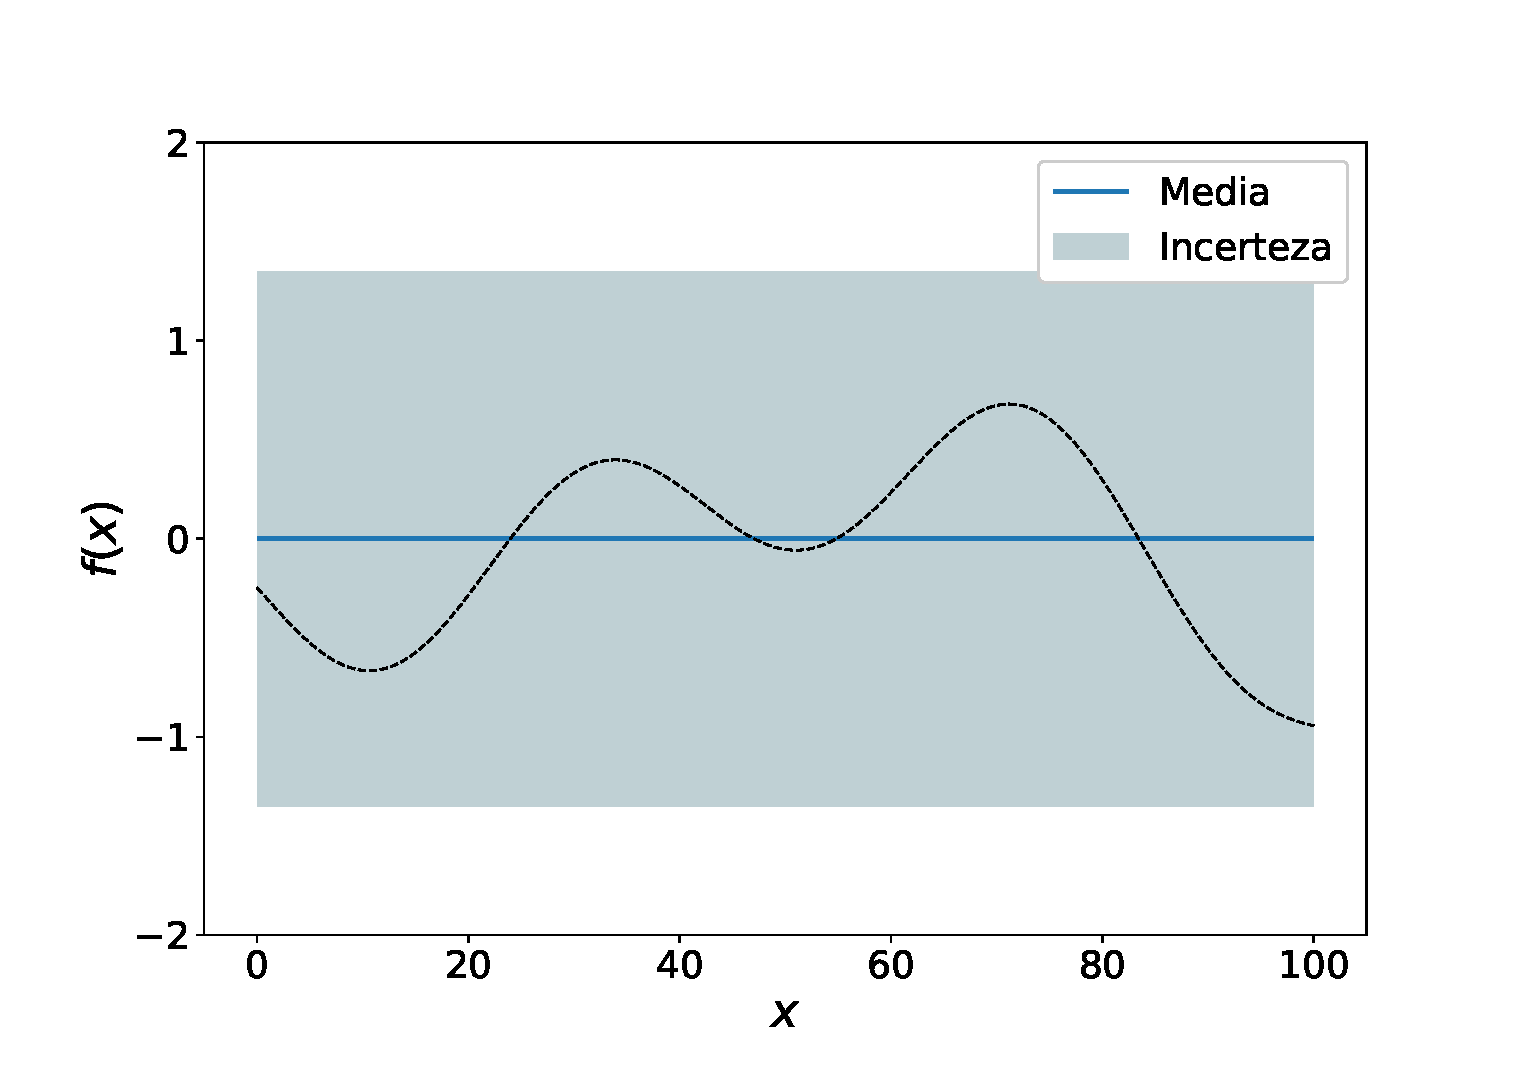
\includegraphics[trim={1.0cm 0 2cm 1cm},clip,height=0.2\textheight]{figures/gp/funcion.eps} 
\includegraphics[trim={3.0cm 0 2cm 1cm},clip,height=0.2\textheight]{figures/gp/func_acq.eps} 
\includegraphics[trim={3.0cm 0 2cm 1cm},clip,height=0.2\textheight]{figures/gp/eval1.eps} \\
\vspace{-0.5cm}
\includegraphics[trim={1.0cm 0 2cm 1cm},clip,height=0.2\textheight]{figures/gp/eval2.eps}
\includegraphics[trim={3.0cm 0 2cm 1cm},clip,height=0.2\textheight]{figures/gp/eval3.eps}
\includegraphics[trim={3.0cm 0 2cm 1cm},clip,height=0.2\textheight]{figures/gp/eval4.eps} \\
\vspace{-0.5cm}
\includegraphics[trim={1.0cm 0 2cm 1cm},clip,height=0.2\textheight]{figures/gp/eval5.eps}
\includegraphics[trim={3.0cm 0 2cm 1cm},clip,height=0.2\textheight]{figures/gp/eval6.eps}
\includegraphics[trim={3.0cm 0 2cm 1cm},clip,height=0.2\textheight]{figures/gp/eval7.eps} 
\caption{Visualización de la optimización de una función arbitraria $f$ 
mediante inferencia por procesos gaussianos.}
\label{fig:visualizacion-gp}
\end{figure}



\newpage
%=======================================================================
\section{Resultados}

En esta Sección presentamos los resultados obtenidos de la optimización
del átomo de berilio con estado de carga neutral. Los resultados son 
presentados y analizados en las siguientes subsecciones: energía 
absoluta, energías de excitación, fuerzas de oscilador y secciones 
eficaces de excitación por impacto de electrón. En el ajuste del blanco 
aplicamos el método de optimización bayesiana con procesos gaussianos, 
descrito en la Sección~\ref{sec:gaussianprocess}, mediante la 
implementación del código GPyOpt~\cite{GPyOpt}.

Como hemos establecido en este capítulo, la descripción de los blancos 
atómicos está determinado por tres variables:
\begin{itemize}
\item las configuraciones electrónicas incluidas en el CI,
\item los potenciales modelos definidos en la ecuación radial de 
Schr\"odinger, y
\item los parámetros de escala que definen dichos potenciales.
\end{itemize}
En el presente trabajo, estudiamos la optimización de la estructura 
atómica del Be en el proceso de excitación por impacto de electrón 
considerando solo la última de estas variables. Para ello, definimos a 
priori las configuraciones electrónicas y los modelos potenciales que
modelan dicha estructura. El modelado de Be, a lo largo de esta Sección,
incluye 27 configuraciones electrónicas: $2s^2$, $2snl$ --tal que 
$n=1$-5 y $l=0$-4--, $2p^2$, y $2pnl$ --siendo $n=3$-5 y $l=0$-4--, 
donde los orbitales $5l$ se han supuesto pseudo-orbitales. Esto resulta 
en un total de 90 términos, donde sólo 19 de ellos son términos 
espectroscópicos. Por otro lado, los potenciales modelos elegidos son 
aquellos que mejor describen, sin ningún tipo de ajuste paramétrico, las 
energías y fuerzas de oscilador. Con este criterio, se determinó 
implementar el potencial STO, más un término de intercambio local, y el 
potencial de correlación core-valencia de Norcross.

La optimización de los potenciales y orbitales fue ejecutada en etapas, 
con el fin de comprender en profundidad este proceso. En primera 
instancia, se ajustaron los parámetros que definen el potencial de 
polarización de Norcross. Luego, fijando los parámetros de Norcross 
resultantes, se procedió a ajustar el potencial STO. Para estudiar el 
efecto de la optimización del potencial de Hartree, este procedimiento 
también fue encarado por partes. Cada una de estas partes considera 
ciertas capas definidas por el número cuántico principal $n$. Así, al 
ajuste del potencial STO consistió en optimizar los orbitales $1s$-$3l$, 
$1s$-$4l$ y $\overline{5l}$.

Los parámetros del modelo bayesiano son consistentes a lo largo de todas 
las optimizaciones de esta Sección; se implementó un mapeo inicial de 
tipo latin hypercube, un kernel RBF y una función de adquisión EI. El 
número de evaluaciones iniciales (o conocimiento previo) sobre el cual el 
modelo basa sus primeras predicciones es, en todos los casos, igual al 
número de parámetros a ajustar. Mientras que el número máximo de 
evaluaciones es 20 veces este número.  Así, si el modelo cuenta con 6 
parámetros a ajustar, el número de evaluaciones iniciales es 6 y el valor
máximo es 120.

%%%%%%%%%%%%%%%%%%%%%%%%%%%%%%%%%%%%%%%%%%%%%%%%%%%%%%%%%%%%%%%%%%%%%%%%%
\subsection{Energía absoluta}
%%%%%%%%%%%%%%%%%%%%%%%%%%%%%%%%%%%%%%%%%%%%%%%%%%%%%%%%%%%%%%%%%%%%%%%%%

La introducción del potencial de polarización de Norcross nos permite
ajustar la energía absoluta del estado fundamental del berilio a su valor 
\textit{experimental}, $E_I=29.336884$ Ry~\cite{NIST}. La ecuación 
(\ref{eq:Norcross-pot}) está compuesta por el conjunto de parámetros 
$\{\alpha_l,\rho_l\}$, donde $l=0,1,2$. Así, se define un espacio 
hiper-paramétrico de seis dimensiones. El parámetro $\alpha$ es la 
polarizabilidad de core. El espacio de búsqueda de esta variable fue 
definido alrededor de su valor experimental \cite{Dalgarno:62,Sitz:71},
%(0.05123~\cite{Dalgarno:62} y 0.05224~\cite{Sitz:71}), 
y dentro de un rango de exploración del 20\%, dado por
\begin{equation}
\boldsymbol\alpha=[0.040-0.060]\,.
\end{equation}
Por otro lado, el parámetro $\rho$ se supone un parámetro de ajuste, por 
lo que nos da más libertad para ajustar la energía de ionización con su 
valor experimental. Así, su rango de exploración fue definido como
\begin{equation}
\boldsymbol\rho=[0.50-1.50]\,.
\end{equation}

La función de costo implementada para ajustar el potencial de 
polarización del core fue definida como
\begin{equation}
J_{\mathrm{pol}} = \sum_{i} \left|\frac{E_{i}-\tilde{E}_{i}
(\boldsymbol{\lambda})}{E_{i}} \right|
\label{eq:Jpol}
\end{equation}
donde $i$ es el índice de los términos incluidos en la optimización, 
$E_{i}$ es la energía absoluta inferida experimentalmente del 
término $i$--ésimo y $\tilde{E}_{i}$ es el valor teórico correspondiente, 
el cual depende de los parámetros $\{\boldsymbol\alpha,\boldsymbol\rho\}$.

El número inicial de evaluaciones fue 6, con un número máximo de 120. Una 
de las grandes dificultades de la minimización u optimización de 
parámetros es la inevitable posibilidad de encontrar un mínimo local. 
Para descartar esta situación, se lanzaron 100 optimizaciones con 
semillas diferentes. Estos cálculos son reveladores, ya que nos permiten 
encontrar relaciones subyacentes entre los parámetros y la naturaleza 
no-convexa de la superficie hiperdimensional definida por $J$.

En la primera optimización (Opt. I), consideramos únicamente la energía
absoluta del estado fundamental $2s^2\,^1S$. El 100\% de los cálculos con
semillas aleatorias encontraron un mínimo para la función de costo menor 
o igual a 0.002\%; mientras que la optimización de 30 semillas 
conducieron a un costo menor o igual a $1\times 10^{-4}$. La 
tabla~\ref{tab:optpol} muestra los mejores resultados de energías 
absolutas hallados para los 11 términos espectroscópicos considerados. 
Si bien la optimización incluye sólo la energía del estado fundamental, 
es de esperar que la representación del resto de los niveles 
espectroscópicos mejore en consecuencia, y es efectivamente lo que se 
observa. Por otro lado, la distribución de los parámetros correspondiente 
a los mínimos muestran una fuerte correlación positiva ($r=0.999$) entre 
$\alpha$ y $\rho$ para $l=0$, mientras que los parámetros para $l=1$ y 
$l=2$ no muestran correlación alguna. Este fenómeno se puede entender 
teniendo en cuenta que sólo el término $2s^2\,^1S$ es incluido en la 
optimización. A pesar de esto, el error relativo de las energías de 
excitación (respecto al estado fundamental) de los 10 términos 
espectroscópicos restantes es menor al 5\%, con excepción de los 
términos $2s2p\,^1P$, $2p^2\,^1D$ y $2s3d\,^1D$.

\begin{table}
\centering
\begin{tabular}{|*{8}{c|}}
\hline 
$i$ & Término & NIST 
  & Sin opt.    & Opt. I     & Opt. II    & Opt. III   & Opt. IV \\
\hline \hline 
\rowcolor{mygray} 
1 & $2s^2\,^1S$ & $-29.3369$ 
  & $-29.2342$  & $-29.3369$ & $-29.3369$ & $-29.3433$ & $29.3426$ \\ & & 
  & $3.5[-1]^\dagger$ & $1.0[-5]$ & $1.0[-4]$ & $2.2[-2]$ & $1.9[-1]$ \\ 
\rowcolor{mygray} 
2 & $2s2p\,^3P$ & $-29.1366$ 
  & $-29.0302$  & $-29.1310$ & $-29.1368$ & $-29.1464$ & $29.1430$ \\ & & 
  & $3.7[-1]$   & $1.9[-2]$  & $7.1[-4]$  & $3.4[-2]$  & $2.2[-1]$ \\ 
\rowcolor{mygray} 
3 & $2s2p\,^1P$ & $-28.9490$ 
  & $-28.8117$  & $-28.9112$ & $-28.9150$ & $-28.9229$ & $28.9210$ \\ & & 
  & $4.7[-1]$   & $1.3[-1]$  & $1.2[-1]$  & $9.0[-2]$  & $9.7[-1]$ \\ 
\rowcolor{mygray}
4 & $2s3s\,^3S$ & $-28.8623$ 
  & $-28.7610$  & $-28.8610$ & $-28.8599$ & $-28.8649$ & $28.8654$ \\ & & 
  & $3.5[-1]$   & $4.3[-3]$  & $8.2[-3]$  & $9.1[-3]$  & $1.1[-1]$ \\ 
\rowcolor{mygray} 
5 & $2s3s\,^1S$ & $-28.8386$ 
  & $-28.7326$  & $-28.8327$ & $-28.8319$ & $-28.8371$ & $28.8374$ \\ & & 
  & $3.7[-1]$   & $2.0[-2]$  & $2.3[-2]$  & $5.5[-3]$  & $4.3[-2]$ \\ 
\rowcolor{mygray} 
6 & $2p^2\,^1D$ & $-28.8185$
  & $-28.5744$  & $-28.6737$ & $-28.8058$ & $-28.8148$ & $28.8119$ \\ & & 
  & $8.5[-1]$   & $5.0[-1]$  & $4.4[-2]$  & $1.3[-2]$  & $2.3[-2]$\\ 
\rowcolor{mygray} 
7 & $2s3p\,^3P$ & $-28.8001$ 
  & $-28.6966$  & $-28.7964$ & $-28.7963$ & $-28.8018$ & $28.8019$ \\ & & 
  & $3.6[-1]$   & $1.3[-2]$  & $1.3[-2]$  & $6.1[-3]$  & $6.2[-2]$ \\  
\rowcolor{mygray} 
8 & $2p\,^3P$   & $-28.7929$ 
  & $-28.6746$  & $-28.7729$ & $-28.7862$ & $-28.8000$ & $28.7932$ \\ & & 
  & $4.1[-1]$   & $6.9[-2]$  & $2.3[-2]$  & $2.5[-2]$  & $1.0[-2]$ \\  
\rowcolor{mygray} 
9 & $2s3p\,^1P$ & $-28.7884$ 
  & $-28.6768$  & $-28.7765$ & $-28.7788$ & $-28.7858$ & $28.7846$ \\ & & 
  & $3.9[-1]$   & $4.2[-2]$  & $3.4[-2]$  & $9.2[-3]$  & $1.3[-2]$ \\  
\rowcolor{mygray} 
10& $2s3d\,^3D$ & $-28.7714$ 
  & $-28.6677$  & $-28.7673$ & $-28.7661$ & $-28.7708$ & $28.7715$ \\ & & 
  & $3.6[-1]$   & $1.4[-2]$  & $1.9[-2]$  & $2.1[-3]$  & $2.8[-4]$ \\  
\rowcolor{mygray} 
11& $2s3p\,^1D$ & $-28.7498$ 
  & $-28.7020$  & $-28.8010$ & $-28.7361$ & $-28.7422$ & $28.7418$ \\ & & 
  & $1.7[-1]$   & $1.8[-1]$  & $4.7[-2]$  & $2.6[-2]$  & $2.8[-2]$ \\ 
\hline\multicolumn{3}{c}{$\,^{\dagger}\,a[b]$ denota $a\times 10^b$} \\
\end{tabular}
\caption[Energías absolutas de Be.]
{Energías absolutas en Rydbergs de los primeros 11 términos 
espectroscópicos de Be (filas superiores) y sus errores relativos 
porcentuales respecto a NIST (filas inferiores).}
\label{tab:optpol}
\end{table}

En la segunda optimización, denominada Opt. II, incluimos los términos 
$2s2p\,^3P^*$ y $2s2p\,^1P^*$ en la función de costo dada por la 
ecuación~(\ref{eq:Jpol}). Así, introducimos además la correlación en los 
parámetros con momento angular $l=1$ del potencial de Norcross. 
Nuevamente, realizamos cálculos independientes con 100 semillas aleatorias. 
Los mínimos hallados por cada uno de estos cálculos tuvieron una 
dispersión menor al 0.01\%. El mejor resultado hallado se muestra en la 
tabla~\ref{tab:optpol}. Esta optimización muestra una mejora tanto para 
las energías absolutas de los términos optimizados como en el resto de 
los niveles espectroscópicos. Los errores relativos de las energías de 
excitación de los 10 términos espectroscópicos fueron menores al 3\% y en 
promedio del 1\%, con excepción del término $2p^2\,^1P$. Además de la 
fuerte correlación entre $\alpha_0$ y $\rho_0$, la inclusión de los 
términos correspondientes a la configuración $2s2p$ introduce en la 
función de costo una fuerte correlación entre $\alpha_1$ y $\rho_1$.

Luego, incluimos los términos $2s3s\,^3S$, $2s3s\,^1S$, y $2p^2\,^1D$ en 
la función de costo (Opt. III). Nuevamente, los mínimos hallados por cada 
uno de los 100 cálculos aleatorios tuvieron una dispersión menor al 
0.01\% alrededor del promedio ($\bar{J}=0.17$). El mejor resultado de 
estos cálculos se muestra en la tabla~\ref{tab:optpol}. Las energías de 
excitación de los 10 términos espectroscópicos en esta optimización 
fueron menores al 2\% y en promedio del 1\%, nuevamente, a excepción del 
término $2p^2\,^1P$. 

Finalmente, incluimos la energía absoluta de los 11 términos 
espectroscópicos en la función de costo (Opt. IV). Los mínimos hallados 
por 100 cálculos de semillas aleatorias, y su distribución en frecuencia, 
se muestran en el panel superior de la figura~\ref{fig:optIV}. Los 
parámetros del potencial de Norcross correspondientes a estos mínimos se 
presentan en el panel inferior de la figura~\ref{fig:optIV}. La 
distribución de los mínimos hallados es tal que la máxima frecuencia de 
se ubica alrededor de su valor medio, $\overline{J}=2.3\times 10^{-1})$, 
con una desviación estándar igual a $\sigma=2.9\times 10^{-3}$. El 50\% 
de los mínimos, que se encuentran por debajo de la media (datos en color 
rojo), tienen parámetros asociados ubicados en la misma region del 
hiper-espacio. Este resultado sugiere que los cálculos independientes con
semillas aleatorias hallaron el mismo mínimo global. Los resultados de la 
mejor optimización bayesiana de $\alpha_l$ y $\rho_l$ se muestran en la 
figura~\ref{fig:globmin}. En el panel superior se presenta la evaluación 
de la función de costo a medida que los procesos gaussianos exploran la
superficie hiper-dimensional de la función de costo. Cada uno de estos 
puntos se corresponde a un punto del espacio de parámetros, que se 
muestra en el panel inferior. El mínimo de la función de costo vecinos es 
hallado en la iteración 81; este punto y sus vecinos más cercanos 
($J\leq 0.245$) se muestran con símbolos de color negro. Los parámetros 
que le corresponden a dichas evaluaciones también se muestran en la parte
inferior con símbolos de color negro.

%%%% Resultados de 100 optimizaciones 
\begin{figure}
\centering
\includegraphics[width=0.85\textwidth]{figures/rmatrix/Jpol_optIV.pdf} \\
\includegraphics[width=0.85\textwidth]{figures/rmatrix/histparams_optIV.pdf}
\caption[Distribución de mínimos y parámetros según semillas aleatorias.]
{(Panel superior) Valores mínimos encontrados para la función de 
costo~(\ref{eq:Jpol}) según 100 cálculos independientes con semillas 
aleatorias (izquierda) y su distribución en frecuencia (derecha).
(Panel inferior) Distribución en frecuencia de los parámetros $\alpha_l$ 
y $\rho_l$ para $l=0,1,2$ correspondientes a los valores mínimos 
hallados.}
%\label{fig:Jpol-optIV}
\label{fig:optIV}
\end{figure}
%\begin{figure}
%\centering
%%\includegraphics[width=0.8\textwidth]{figures/rmatrix/params_optIV.pdf}
%\caption[Distribución de parámetros según semillas aleatorias.]
%{Distribución en frecuencia de los parámetros $\alpha_l$ y $\rho_l$ 
%($l=0,1,2$) correspondientes a los valores mínimos que se muestran en la 
%figura~(\ref{fig:Jpol-optIV}).}
%\label{fig:params-optIV}
%\end{figure}

%%%% Resultados de la mejor optimización
\begin{figure}
\centering
\includegraphics[width=0.85\textwidth]{figures/rmatrix/Jpol_globmin.pdf}
\includegraphics[width=0.85\textwidth]{figures/rmatrix/params_globmin.pdf}
\caption[Minimización de la función de costo y exploración de parámetros.]
{(Panel superior) Optimización bayesiana de la función de costo dada por 
la ecuación~(\ref{eq:Jpol}). (Panel inferior) Exploración del 
hiper-espacio de parámetros correspondiente.}
%\label{fig:Jpol-globmin}
\label{fig:globmin}
\end{figure}
%\begin{figure}
%\centering
%\includegraphics[width=0.8\textwidth]{figures/rmatrix/params_globmin.pdf}
%\caption[Exploración del espacio de parámetros.]
%{Exploración del espacio de parámetros correspondiente a la minimización
%dada en la figura~(\ref{fig:Jpol-globmin}).}
%\label{fig:params-globmin}
%\end{figure}

%%%%%%%%%%%%%%%%%%%%%%%%%%%%%%%%%%%%%%%%%%%%%%%%%%%%%%%%%%%%%%%%%%%%%%%%%
\subsection{Energías de excitación}
%%%%%%%%%%%%%%%%%%%%%%%%%%%%%%%%%%%%%%%%%%%%%%%%%%%%%%%%%%%%%%%%%%%%%%%%%

En esta sección estudiamos la optimización de las energías de excitación 
respecto al estado fundamental. Esta optimización consiste en ajustar los 
parámetros $\lambda_{nl}$ que definen al potencial modelo STO de manera
tal que las energías de los términos espectroscópicos del Be se ajusten 
a los datos experimentales~\cite{NIST}. En esta optimización se mantiene 
constante los parámetros del potencial de Norcross hallados en la 
optimización IV de la sección anterior.

La optimización del potencial STO también se presenta por partes. En 
primera instancia, denominada Opt. A, se ajustaron los orbitales $1s$, 
$2s$, $2p$, $3s$, $3p$ y $3d$. La segunda optimización, Opt.~B, incluyó
la variación de 10 orbitales $nl$, desde $1s$ hasta $4f$. Por último, se 
ajustaron los parámetros que definen los pseudo-orbitales 
$\overline{5s}$, $\overline{5p}$, $\overline{5d}$, $\overline{5f}$ y 
$\overline{5g}$. En esta optimización, denominada Opt.~C, se mantuvieron 
constantes los parámetros $\lambda_{nl}$ encontrados en Opt.~B. Los 
resultados de estas tres optimizaciones se presentan en la 
tabla~\ref{tab:exener}. En todos los casos, la función de costo considera 
las energías absolutas de los primeros 11 términos espectroscópicos. La 
energía absoluta del estado fundamental halladas en las optimizaciones 
A, B y C fueron $-29.335167$~Ry, $-29.33772$~Ry, $-29.337362$~Ry, 
respectivamente, lo que representa una error relativo del 
$6\times 10^{-3}\%$, $4\times 10^{-3}\%$ y $2\times 10^{-3}\%$ respecto 
al valor conocido. Una mejor visualización de los resultados de la 
tabla~\ref{tab:exener} se presentan en la figura~\ref{fig:exener}, donde 
se dan los errores relativos de las energías de excitación consideradas 
y sus valores medios (líneas discontinuas). Los valores de las energías 
de excitación respecto al estado fundamental son mejoradas 
sistemáticamente con las optimizaciones a medida que se aumenta el número 
de parámetros, i.e. orbitales a ajustar. Así, el error relativo promedio 
se reduce hasta un orden de magnitud respecto al modelo atómico sin 
optimizar. Los términos más afectados por la optimización fueron 
$2s2p\,^1P^*$, $2p^2\,^1D$ y $2s3d\,^1D$, que presentan una desviación 
(sin optimización) del 9\%, 27\% y 9\%, respectivamente. El ajuste de los 
orbitales espectroscópicos (Opt. B) y los pseudo-orbitales (Opt. C) 
reducen estos valores por debajo de 2\%, con un promedio del $0.6\%$. Si 
bien ambas optimizaciones mejoran significativamente la representación de 
los niveles espectroscópicos, vale remarcar que el orden resultante de 
los términos $2p^2\,^3P$ y $2s3p\,^1P$ se encuentran invertidos. La 
incorrecta representación de estos niveles podría ser mejorada, por 
ejemplo, considerando un mayor número de configuraciones que intervengan 
en el CI de estos términos.

{\color{red} Falta dar detalle respecto a la optimización C.}

\begin{table}
\centering
\begin{tabular}{|*{7}{c|}}
\hline 
$i$ & Término & NIST & Sin opt. & Opt. A & Opt. B & Opt. C \\
\hline 
\hline 
1 & $2s^2\,^1S$   & $0.0000$ & $0.0000$ & $0.0000$ & $0.0000$ & $0.0000$ \\
2 & $2s2p\,^3P^*$ & $0.2003$ & $0.2040$ & $0.1987$ & $0.1998$ & $0.1976$ \\
3 & $2s2p\,^1P^*$ & $0.3879$ & $0.4225$ & $0.4185$ & $0.3952$ & $0.3947$ \\
4 & $2s3s\,^3S$   & $0.4746$ & $0.4732$ & $0.4729$ & $0.4714$ & $0.4724$ \\
5 & $2s3s\,^1S$   & $0.4983$ & $0.5016$ & $0.4972$ & $0.4991$ & $0.4985$ \\
6 & $2p^2\,^1D$   & $0.5184$ & $0.6598$ & $0.5296$ & $0.5181$ & $0.5161$ \\
7 & $2s3p\,^3P^*$ & $0.5368$ & $0.5376$ & $0.5345$ & $0.5368$ & $0.5369$ \\
8 & $2p^2\,^3P$   & $0.5440$ & $0.5595$ & $0.5476$ & $0.5537$ & $0.5503$ \\
9 & $2s3p\,^1P^*$ & $0.5485$ & $0.5574$ & $0.5546$ & $0.5493$ & $0.5501$ \\
10 & $2s3d\,^3D$  & $0.5655$ & $0.5665$ & $0.5642$ & $0.5639$ & $0.5647$ \\
11 & $2s3d\,^1D$  & $0.5871$ & $0.5322$ & $0.5924$ & $0.5877$ & $0.5873$ \\
\hline
\end{tabular}
\caption[Energías de excitación de Be.]
{Energía de excitación en Rydbergs de los primeros 11 términos 
espectroscópicos de Be relativos al estado fundamental $2s^2\,^1S$.}
\label{tab:exener}
\end{table}
\begin{figure}
\centering
\includegraphics[width=0.85\textwidth]{figures/rmatrix/erp_ei.pdf} 
\caption[Error relativo de 10 términos espectroscópicos de Be.]
{Error relativo de los primeros 10 términos espectroscópicos respecto 
a valores de NIST. Las líneas discontinuas representan el error relativo
porcentual promedio de cada cálculo.}
\label{fig:exener}
\end{figure}

%%%%%%%%%%%%%%%%%%%%%%%%%%%%%%%%%%%%%%%%%%%%%%%%%%%%%%%%%%%%%%%%%%%%%%%%%
\subsection{Fuerzas de oscilador de asborción}

En esta sección presentamos las fuerzas de oscilador de absorción 
resultantes de las optimizaciones del potencial STO, calculadas en el 
\textit{gauge} de longitud, para un conjunto de transiciones en Be. 
Nuestros resultados son comparados con valores experimentales~\cite{NIST} 
en la tabla~\ref{tab:fabs}. Los errores relativos correspondientes se 
presentan en la figura~\ref{fig:fabs}, donde se observa una mejora 
significativa en la representación de las transiciones 
$2s^2\,^1S\rightarrow 2s3p\,^1P$, $2s2p\,^1P\rightarrow 2s3s\,^1S$, 
$2s2p\,^1P\rightarrow 2s3d\,^1D$, y $2s3p\,^1P\rightarrow 2s3d\,^1D$.
Los resultados sin optimizar tienen un error relativo de aproximadamente  
84\%, mientras que las optimizaciones B y C presentan errores relativos 
promedios similares, ambas menores al 14\%. Si bien la función de costo
sólo considera los valores de energía de los términos espectroscópicos,
es notable la mejora en la representación de este grupo de transiciones 
dipolares.

\begin{table}
\begin{adjustwidth}{-.6in}{-.6in}  
\centering
%\begin{tabular}{|*{9}{c|}} 
\begin{tabular}{|*{7}{c|}} 
\hline 
No & Transición &
NIST &
%Ballance   & Chen       & MCHF       & 
Sin opt.   & Opt. A    & Opt. B  & Opt. C\\
\hline
\hline
1  & $2s^2  \,^1S - 2s2p \,^1P$ & 
$1.37$ &
%$1.37$     & $1.38$     & $1.38    $ & 
$1.32    $ & $1.31    $ & $1.40    $ & $1.38$ \\
%%%%
2  & $2s^2  \,^1S - 2s3p \,^1P$ & 
$8.98[-3]$ &
%$1.12[-2]$ & $9.01[-3]$ & $8.99[-3]$ &
$5.70[-2]$ & $5.84[-2]$ & $1.71[-2]$ & $1.55[-2]$ \\
%%%%
3  & $2s2p \,^3P - 2s3s \,^3S$ & 
$8.44[-2]$ &
%$7.56[-2]$ & $8.23[-2]$ & $8.41[-2]$ & 
$8.57[-2]$ & $8.22[-2]$ & $8.49[-2]$ & $8.21[-2]$ \\
%%%%
4  & $2s2p \,^3P - 2s3d \,^3D$ & 
$2.99[-1]$ &
%$2.99[-1]$ & $2.95[-1]$ & $3.00[-1]$ & 
$2.96[-1]$ & $2.67[-1]$ & $3.08[-1]$ & $2.96[-1]$ \\
%%%%
5  & $2s2p \,^1P - 2s3s \,^1S$ & 
$1.15[-1]$ &
%$1.20[-1]$ & $1.18[-1]$ & $1.15[-1]$ & 
$1.62[-1]$ & $1.59[-1]$ & $1.23[-1]$ & $1.29[-1]$ \\
%%%%
6  & $2s2p \,^1P - 2s3d \,^1D$ & 
$3.98[-1]$ &
%$3.86[-1]$ & $4.10[-1]$ & $3.96[-1]$ & 
$8.18[-2]$ & $2.20[-1]$ & $3.83[-1]$ & $3.74[-1]$ \\
%%%%
7  & $2s3s \,^3S - 2s3p \,^3P$ & 
$1.13$ &
%$1.02$     & $1.13    $ & $1.14    $ & 
$1.15    $ & $1.10$     & $1.13    $ & $1.12$ \\
%%%%
8  & $2s3s \,^1S - 2s3p \,^1P$ & 
$9.57[-1]$ &
%$9.08[-1]$ & $9.58[-1]$ & $9.47[-1]$ & 
$9.02[-1]$ & $8.99[-1]$ & $9.80[-1]$ & $9.87[-1]$ \\
%%%%
%9  & $2s3p \,^3P - 2s3d \,^3D$ & 
% &
%%$4.83[-1]$ & $5.01[-1]$ & $5.14[-1]$ & 
%$4.92[-1]$ & $5.08[-1]$ & $4.91[-1]$ & $5.18[-1]$ \\
%%%%
9 & $2s3p \,^1P - 2s3d \,^1D$ & 
$6.78[-1]$ &
%$6.91[-1]$ & $6.87[-1]$ & $6.81[-1]$ & 
$9.26[-2]$ & $7.74[-1]$ & $7.70[-1]$ & $7.99[-1]$ \\
\hline
\end{tabular}
\caption{Fuerza de oscilador de absorción de transiciones dipolares en 
Be.}
\label{tab:fabs}
\end{adjustwidth}
\end{table}
\begin{figure}
\centering
\includegraphics[width=0.9\textwidth]{figures/rmatrix/erp_fabs.pdf} 
\caption{Error relativo de fuerzas de oscilador de absorción dipolares 
correspondientes a la tabla~\ref{tab:fabs}.}
\label{fig:fabs}
\end{figure}

%%%%%%%%%%%%%%%%%%%%%%%%%%%%%%%%%%%%%%%%%%%%%%%%%%%%%%%%%%%%%%%%%%%%%%%%%
\subsection{Excitación por impacto de electrón}

Los resultados obtenidos del cálculo de las secciones eficaces de 
excitación por impacto de electrón en Be se muestran en las 
figuras~\ref{fig:crossBe-partI} y \ref{fig:crossBe-partII}. Las figuras 
muestran las secciones eficaces obtenidas cuando se ajustaron con 
distintas aproximaciones la estructura atómica del Be: sin optimización, 
y las optimizaciones A, B y C de los parámetros $\lambda_{nl}$. Nuestros
resultados se comparan con secciones eficaces de referencia: las líneas
negras discontinuas~\cite{Dipti:19} corresponden a promedios de los 
mejores resultados de la literatura, y se toman como referencia. También
incluimos los valores predichos por el método CCC~\cite{Fursa:97} 
(símbolos circulares), los cuales son considerados en la expresión 
paramétrica dada por~\cite{Dipti:19}. Las transiciones del estado 
fundamental a los primeros 7 estados excitados son ligeramente mejorados 
a partir de las sucesivas optimizaciones, a excepción de la transición 
$2s^2\,^1S\rightarrow 2p^2\,^1D$. Cuando el blanco no está optimizado, 
la sección eficaz de excitación en esta transición está por debajo de 
las predicciones de referencia en la región intermedia. La influencia de 
la optimización del blanco es significativa en los términos 
espectroscópicos más altos. Por ejemplo, en la transición 
$2s^2\,^1S\rightarrow 2s3s\,^1P$, la sección eficaz predicha cuando el 
blanco no está optimizado es el doble que los valores de referencia a lo 
largo de todo el rango de energía. Se puede observar que las sucesivas 
optimizaciones permiten converger a los valores de referencia y 
reproducir las secciones eficaces de excitación con precisión en todas
las transiciones inspeccionadas. 

\begin{figure}
\centering
\includegraphics[width=0.9\textwidth]{figures/rmatrix/GP_RMPS_x6.eps} 
\caption[Secciones eficaces de excitación de Be (Parte I).]
{(Parte I) Secciones eficaces de excitación por impacto de electrón en Be. 
Curvas: Dipti \textit{et al.}~\cite{Dipti:19} (discontinua), RMPS sin 
ajuste (punteada); cálculos con ajuste: Opt. A (raya-punto), Opt. B 
(raya-punto-punto), y Opt. C (continua). 
Símbolos: cálculos CCC de \cite{Fursa:97}.}
\label{fig:crossBe-partI}
\end{figure}

\begin{figure}
\centering
\includegraphics[width=0.9\textwidth]{figures/rmatrix/GP_RMPS_x4.eps} 
\caption[Secciones eficaces de excitación de Be (Parte II).]
{(Parte II) Secciones eficaces de excitación por impacto de electrón en Be.
Curvas y símbolos: iguales a figura~\ref{fig:crossBe-partI}.}
\label{fig:crossBe-partII}
\end{figure}

\newpage
%=======================================================================
\section{Conclusiones}
